\documentclass[12pt,a4paper]{article}
\usepackage[utf8]{inputenc}
\usepackage[spanish,es-tabla]{babel}
\usepackage{geometry}
\usepackage{graphicx}
\usepackage{multirow}
\usepackage{tabularx}
\usepackage{mathptmx}
\usepackage{fancyhdr}
\usepackage{array}
\usepackage[table]{xcolor}
\usepackage{titlesec}
\usepackage{setspace}
\usepackage{microtype}
\usepackage{lastpage}
\usepackage{booktabs}
\usepackage{enumitem}
\usepackage{amsmath}
\usepackage{amsfonts}
\usepackage{amssymb}

\usepackage{float}
\usepackage{placeins}
\usepackage{tikz}
\usepackage{pgfplots}
\pgfplotsset{compat=1.17}
\usetikzlibrary{arrows.meta,positioning,shapes.geometric,calc}

\graphicspath{{images/}{../images/}{./}}

\geometry{
    top=4.7cm,
    bottom=2.5cm,
    left=2.5cm,
    right=2.5cm,
    headheight=3.9cm,
    headsep=0.4cm
}

\setstretch{1.15}
\setlength{\parindent}{0pt}
\setlength{\parskip}{0.45em}
\setlength{\tabcolsep}{4pt}

\titleformat{\section}
  {\normalfont\fontsize{12}{14.5}\bfseries}{\thesection.}{0.6em}{\uppercase}
\titlespacing*{\section}
  {0pt}{1.8ex plus 0.4ex minus 0.2ex}{0.6ex plus 0.2ex}

\titleformat{\subsection}
  {\normalfont\fontsize{11.5}{13.5}\bfseries}{\thesubsection.}{0.5em}{}
\titlespacing*{\subsection}
  {0pt}{1.4ex plus 0.3ex minus 0.1ex}{0.4ex plus 0.1ex}

\titleformat{\subsubsection}
  {\normalfont\fontsize{10.5}{12.5}\bfseries\itshape}{\thesubsubsection.}{0.4em}{}
\titlespacing*{\subsubsection}
  {0pt}{1.1ex plus 0.2ex minus 0.1ex}{0.3ex plus 0.1ex}

\newcolumntype{Y}{>{\centering\arraybackslash}X}
\newcolumntype{L}{>{\raggedright\arraybackslash}X}
\newcolumntype{C}{>{\centering\arraybackslash}X}

\definecolor{headerblue}{RGB}{26, 54, 93}
\definecolor{darkblue}{RGB}{43, 108, 176}
\definecolor{lightgraybg}{RGB}{248, 248, 248}
\definecolor{tableheader}{RGB}{232, 238, 246}
\definecolor{navyheader}{RGB}{0, 32, 96}
\definecolor{lineblue}{RGB}{0, 102, 204}
\definecolor{areablue}{RGB}{220, 236, 252}
\definecolor{lcsred}{RGB}{217, 56, 41}
\definecolor{lcigreen}{RGB}{46, 125, 50}
\definecolor{lciorange}{RGB}{230, 81, 0}
\definecolor{ishikawared}{RGB}{160, 0, 0}

\tikzset{
    catbox/.style={draw, fill=tableheader, font=\footnotesize\bfseries, minimum width=2.8cm, minimum height=0.65cm, align=center},
    efectobox/.style={draw=ishikawared!90!black, line width=1.2pt, fill=ishikawared, text=white, font=\small\bfseries, align=center, inner sep=6pt, text width=3.8cm},
    causetext/.style={font=\scriptsize, align=right, text=black!90}
}

\newcommand{\docCodigo}{TI-SIGE-ENT-F1-008}
\newcommand{\docVersion}{1.0}
\newcommand{\docProceso}{ASEGURAMIENTO DE CALIDAD / HITO DE CONTROL 1}
\newcommand{\docElaboracion}{24/08/2026}
\newcommand{\docRevision}{24/08/2026}
\newcommand{\docTitulo}{HITO 1: APROBACIÓN DE FASE 1 Y ENTREGABLE GENERAL SEMANA 1}
\newcommand{\docOrganizacion}{FACULTAD DE INGENIERÍA EN SISTEMAS, ELECTRÓNICA E INDUSTRIAL}
\newcommand{\docSubOrganizacion}{CARRERA DE INGENIERÍA DE SOFTWARE}

\newcommand{\encabezadofrecuente}{%
    \renewcommand{\arraystretch}{1.15}%
    \noindent\makebox[\textwidth][c]{%
    \begin{tabularx}{\textwidth}{|>{\centering\arraybackslash}m{2.8cm}|Y|>{\centering\arraybackslash}m{4.8cm}|}
        \hline
        \multirow{4}{2.8cm}{\centering\raisebox{-1.15cm}{
\includegraphics[width=2.5cm,height=2.0cm,keepaspectratio]{images/logo.png}}}
        & \textbf{\fontsize{9}{11}\selectfont \docOrganizacion} 
        & \textbf{\fontsize{8}{10}\selectfont CÓDIGO:} \fontsize{8}{10}\selectfont \docCodigo \\
        \cline{3-3}
        & \textbf{\fontsize{8.5}{10.5}\selectfont \docSubOrganizacion} 
        & \textbf{\fontsize{8}{10}\selectfont VERSIÓN:} \fontsize{8}{10}\selectfont \docVersion \\
        \cline{2-3}
        & \textbf{\fontsize{8}{10}\selectfont PROCESO:} \fontsize{8}{10}\selectfont \docProceso 
        & \textbf{\fontsize{8}{10}\selectfont ELABORACIÓN:} \fontsize{8}{10}\selectfont \docElaboracion \\
        \cline{2-3}
        & \textbf{\fontsize{8.5}{10.5}\selectfont \docTitulo} 
        & \textbf{\fontsize{8}{10}\selectfont ÚLTIMA REVISIÓN:} \fontsize{8}{10}\selectfont \docRevision \\
        \hline
    \end{tabularx}%
    }%
}

\pagestyle{fancy}
\fancyhf{}
\fancyhead[C]{\encabezadofrecuente}
\fancyfoot[C]{\fontsize{10}{12}\selectfont Página \thepage\ de \pageref{LastPage}}
\renewcommand{\headrulewidth}{0pt}

\begin{document}

\noindent{\fontsize{10.5}{12.5}\selectfont \textbf{Integrantes:} Heidi Villavicencio \quad$\vert$\quad Steeven Toala \quad$\vert$\quad Nixon Hurtado \quad$\vert$\quad Andrea Vásquez}

\vspace{0.25cm}

\section{Título}
\textbf{Denominación Oficial del Entregable:} HITO 1: Aprobación de Fase 1 y Entregable General Semana 1 -- Código EDT: 1.8

\section{Introducción}
El cierre formal de la Fase 1: Análisis y Planificación del proyecto SIGE representa la culminación exitosa de las actividades de diagnóstico As-Is, ingeniería de requerimientos, modelado de compuertas lógicas, evaluación financiera y estructuración del cronograma maestro. El presente informe formaliza la revisión colegiada y aprobación del Hito 1 ante el docente asesor y evaluador Ing. Paulo Torres. Se consolida la trazabilidad de los 7 entregables predecesores (EDT 1.1 al 1.7) y se incorporan las tres herramientas analíticas de control de calidad exigidas institucionalmente: el Diagrama de Causa-Efecto de Ishikawa, el Diagrama de Comportamiento (Run Chart) y el Gráfico de Trabajo Completado (Burnup Chart), demostrando el cumplimiento estricto del 100\% de las metas de la fase.

\section{Objetivo}
\subsection{Objetivo General}
Consolidar, evaluar y aprobar formalmente el paquete de entregables de la Fase 1: Análisis y Planificación (Hito 1), certificando la conformidad técnica, analítica y metodológica para el paso a la Fase 2 de Diseño y Arquitectura.
\subsection{Objetivos Específicos}
\begin{itemize}[leftmargin=1.5em, itemsep=2pt]
    \item Verificar el cumplimiento y calidad técnica de los entregables EDT 1.1 al 1.7.
    \item Documentar el análisis de causa-efecto mediante el Diagrama de Ishikawa de cuellos de botella SGC.
    \item Evaluar el comportamiento operativo con el Run Chart y el ritmo de trabajo acumulado con el Burnup Chart.
    \item Suscribir el acta formal de aprobación de Hito 1 por parte del docente evaluador.
\end{itemize}

\section{Alcance}
\subsection{Límites del Entregable (In-Scope)}
\begin{itemize}[leftmargin=1.5em, itemsep=2pt]
    \item Paquete consolidado de 8 entregables de Fase 1 (12 al 24 de agosto de 2026).
    \item Certificación formal de la línea base del alcance y cronograma.
\end{itemize}
\subsection{Exclusiones (Out-of-Scope)}
\begin{itemize}[leftmargin=1.5em, itemsep=2pt]
    \item Modificaciones a los requisitos ya congelados tras la firma de este hito.
\end{itemize}

\section{Definiciones}
\begin{itemize}[leftmargin=1.5em, itemsep=2pt]
    \item \textbf{Hito de Control (Milestone):} Evento de control con duración de 0 días que certifica la conclusión formal de una fase.
    \item \textbf{Diagrama de Ishikawa:} Herramienta de calidad para representar sistemáticamente causas y subcausas agrupadas en 6 categorías metodológicas.
    \item \textbf{Run Chart:} Gráfico de series temporales que evalúa tendencias y estabilidad de desempeño frente a límites operativos.
    \item \textbf{Burnup Chart:} Gráfico de seguimiento que muestra el avance acumulado de trabajo frente a la línea base del alcance.
\end{itemize}

\section{Responsabilidades}
\begin{itemize}[leftmargin=1.5em, itemsep=2pt]
    \item \textbf{Equipo de Proyecto SIGE (ST, HV, NH, AV - EDT 1.8):} Consolidación del informe, sustentación técnica y demostración de artefactos.
    \item \textbf{Ing. Paulo Torres (Docente Evaluador / Patrocinador):} Revisión exhaustiva de conformidad, retroalimentación y suscripción formal de aprobación.
\end{itemize}

\section{Normativa Legal y Técnica}
\subsection{Marco Legal Ecuatoriano}
\begin{itemize}[leftmargin=1.5em, itemsep=2pt]
    \item \textbf{LOES, Art. 122:} Rendición de cuentas periódica y control de calidad en la docencia universitaria.
\end{itemize}

\subsection{Normas Técnicas Internacionales}
\begin{itemize}[leftmargin=1.5em, itemsep=2pt]
    \item \textbf{Guía PMBOK (7ma Edición), Cierre de Fase:} Procedimientos formales de revisión y aceptación de entregables.
    \item \textbf{ISO 9001:2015, Cláusula 9.1 (Seguimiento, Medición, Análisis y Evaluación):} Análisis de datos de calidad del proceso documental.
\end{itemize}

\section{Método, Políticas y Contenidos}
\subsection{Consolidación de Entregables de Fase 1}
En la reunión formal del 24 de agosto de 2026, el docente evaluador auditó los 7 entregables predecesores, verificando su total conformidad técnica según la Tabla \ref{tab:cierre_fase1}.

\begin{table}[H]
\centering
\small
\renewcommand{\arraystretch}{1.2}
\begin{tabularx}{\textwidth}{|c|>{\bfseries}m{4.0cm}|X|c|c|}
\hline
\rowcolor{tableheader}
\textbf{EDT} & \textbf{Entregable Oficial} & \textbf{Artefacto Verificado} & \textbf{Horas} & \textbf{Estado} \\
\hline
1.1 & Diagnóstico As-Is & Mapeo As-Is y matriz de problemas P-01 a P-06 & 24 h & Aprobado \\
\hline
1.2 & Actores y Procesos & Matriz de Stakeholders y asignación RACI & 32 h & Aprobado \\
\hline
1.3 & Especificación SRS & 24 RFs y 8 RNFs bajo IEEE 830 y trazabilidad & 40 h & Aprobado \\
\hline
1.4 & Alcance y Restricciones & Fronteras del sistema y objetivos SMART & 32 h & Aprobado \\
\hline
1.5 & Reglas y Validation Gates & Especificación de compuertas lógicas RN-01 a RN-10 & 32 h & Aprobado \\
\hline
1.6 & Caso de Negocio y ROI & Presupuesto (\$630.30), ROI (+3,438\%) y Charter & 24 h & Aprobado \\
\hline
1.7 & Cronograma Maestro & EDT 49 tareas, MS Project (57 días, 456h) & 24 h & Aprobado \\
\hline
1.8 & Hito 1: Aprobación Fase 1 & Paquete Completo Aprobado y Análisis Calidad & 0 h & Aprobado \\
\hline
\multicolumn{3}{|r|}{\textbf{TOTAL HORAS INVERTIDAS EN FASE 1:}} & \textbf{208 h} & \textbf{100\%} \\
\hline
\end{tabularx}
\caption{Matriz de Conformidad y Cierre de Entregables de Fase 1.}
\label{tab:cierre_fase1}
\end{table}
\FloatBarrier

\section{Descripción de actividades}

\subsection{Herramienta Analítica 1: Diagrama de Causa y Efecto (Ishikawa)}
Para diagnosticar la raíz del problema central del SGC en la FISEI, se organizaron las causas en 6 categorías metodológicas: Método, Personas, Materiales, Tecnología, Entorno y Medición. La Figura \ref{fig:ishikawa_vector} presenta el modelo vectorial de Ishikawa implementado para SIGE.

\begin{figure}[H]
    \centering
    \resizebox{\textwidth}{!}{%
    \begin{tikzpicture}[
        catbox/.style={
            draw=navyheader, 
            line width=1.1pt, 
            fill=tableheader, 
            font=\footnotesize\bfseries, 
            minimum width=2.7cm, 
            minimum height=0.75cm, 
            align=center
        },
        efectobox/.style={
            draw=ishikawared!90!black, 
            line width=1.2pt, 
            fill=ishikawared, 
            text=white, 
            font=\small\bfseries, 
            align=center, 
            inner sep=7pt, 
            text width=3.9cm
        },
        causetext/.style={
            font=\scriptsize, 
            align=right, 
            text=black!90
        }
    ]
        % 1. Espina Dorsal Central
        \draw[line width=2.4pt, -{Stealth[length=5.5mm, width=4mm]}, draw=black] (0,0) -- (13.0,0);
        
        % Caja de Efecto (Problema Central)
        \node[efectobox, anchor=west] at (13.2, 0) {%
            \textbf{Ineficiencia y falta}\\[2.5pt]%
            \textbf{de trazabilidad en}\\[2.5pt]%
            \textbf{planes e informes SGC}%
        };

        % 2. RAMAS SUPERIORES
        % --- MÉTODO ---
        \node[catbox] (c_metodo) at (2.6, 3.2) {Método};
        \draw[line width=1.4pt, draw=black] (2.6, 2.75) -- (4.6, 0);
        \node[causetext, anchor=east] at (2.82, 2.15) {Ciclos de devolución\\[1pt]por correo y WhatsApp};
        \node[causetext, anchor=east] at (3.36, 1.4) {Reproceso completo desde\\[1pt]Word en cada vuelta};
        \node[causetext, anchor=east] at (3.90, 0.65) {Plan e Informe como\\[1pt]archivos separados};

        % --- PERSONAS ---
        \node[catbox] (c_personas) at (6.6, 3.2) {Personas};
        \draw[line width=1.4pt, draw=black] (6.6, 2.75) -- (8.6, 0);
        \node[causetext, anchor=east] at (6.82, 2.15) {Cálculo de pondera-\\[1pt]ciones con calculadora};
        \node[causetext, anchor=east] at (7.36, 1.4) {Revisión aritmética man-\\[1pt]ual del Coordinador};
        \node[causetext, anchor=east] at (7.90, 0.65) {Fechas redactadas a mano};

        % --- MATERIALES ---
        \node[catbox] (c_materiales) at (10.6, 3.2) {Materiales};
        \draw[line width=1.4pt, draw=black] (10.6, 2.75) -- (12.6, 0);
        \node[causetext, anchor=east] at (10.82, 2.15) {Plantillas Word\\[1pt]y Excel estáticas};
        \node[causetext, anchor=east] at (11.36, 1.4) {Varias versiones\\[1pt]del mismo informe};
        \node[causetext, anchor=east] at (11.90, 0.65) {Matrices sin vali-\\[1pt]dación de ponderación};

        % 3. RAMAS INFERIORES
        % --- TECNOLOGÍA ---
        \node[catbox] (c_tec) at (2.6, -3.2) {Tecnología};
        \draw[line width=1.4pt, draw=black] (2.6, -2.75) -- (4.6, 0);
        \node[causetext, anchor=east] at (3.91, -0.65) {Sin sello de tiempo\\[1pt]del servidor};
        \node[causetext, anchor=east] at (3.36, -1.4) {Evidencias en car-\\[1pt]petas locales o Drive};
        \node[causetext, anchor=east] at (2.82, -2.15) {Sin plataforma centralizada};

        % --- ENTORNO ---
        \node[catbox] (c_entorno) at (6.6, -3.2) {Entorno};
        \draw[line width=1.4pt, draw=black] (6.6, -2.75) -- (8.6, 0);
        \node[causetext, anchor=east] at (7.91, -0.65) {Catálogos de activi-\\[1pt]dades dispersos por área};
        \node[causetext, anchor=east] at (7.36, -1.4) {Tiempos de es-\\[1pt]pera entre etapas};
        \node[causetext, anchor=east] at (6.82, -2.15) {Tres actores y tres\\[1pt]firmas secuenciales};

        % --- MEDICIÓN ---
        \node[catbox] (c_medicion) at (10.6, -3.2) {Medición};
        \draw[line width=1.4pt, draw=black] (10.6, -2.75) -- (12.6, 0);
        \node[causetext, anchor=east] at (11.91, -0.65) {Sin indicadores de\\[1pt]tiempo por informe};
        \node[causetext, anchor=east] at (11.36, -1.4) {Sin auditoría de evidencias};
        \node[causetext, anchor=east] at (10.82, -2.15) {Sin trazabilidad\\[1pt]en tiempo real};
    \end{tikzpicture}%
    }
    \caption{Diagrama de Causa y Efecto (Ishikawa) Vectorial del Proceso Actual SGC en la FISEI.}
    \label{fig:ishikawa_vector}
\end{figure}
\FloatBarrier

\begin{table}[H]
\centering
\small
\renewcommand{\arraystretch}{1.2}
\begin{tabularx}{\textwidth}{|>{\raggedright\arraybackslash\bfseries}m{2.5cm}|X|c|>{\raggedright\arraybackslash}m{3.2cm}|}
\hline
\rowcolor{tableheader}
\textbf{Categoría} & \textbf{Causas Raíz Identificadas (Hechos del Proceso As-Is)} & \textbf{Problema} & \textbf{Solución en SIGE} \\
\hline
\textbf{Método} & Devoluciones informales por correo y WhatsApp; reprocesos completos desde Word; desconexión entre plan e informe. & P-01, P-06 & Flujo web guiado y migración automática de actividades de plan a informe. \\
\hline
\textbf{Personas} & Cálculo aritmético manual de horas y ponderaciones; revisión visual propensa a error; fechas tipeadas a mano. & P-03, P-05 & Reglas automáticas en interfaz y compuerta lógica de suma 100\% obligatoria. \\
\hline
\textbf{Materiales} & Uso de formatos ofimáticos estáticos expuestos a alteración estructural y pérdida de formato. & P-01, P-03 & Plantillas dinámicas protegidas y exportación oficial en PDF y Word idénticos. \\
\hline
\textbf{Tecnología} & Ausencia de plataforma centralizada; evidencias almacenadas en discos locales o enlaces de Drive caídos. & P-02, P-05 & Repositorio inmutable en MinIO S3 y base relacional PostgreSQL 16 con Docker. \\
\hline
\textbf{Entorno} & Dependencia de tres firmas físicas secuenciales; esperas de hasta 15 días hábiles por trámite. & P-04 & Notificaciones por correo, panel de pendientes y firma electrónica en cascada. \\
\hline
\textbf{Medición} & Inexistencia de bitácoras de auditoría y falta de trazabilidad en tiempo real. & P-02, P-04 & Trazabilidad inmutable de cambios, log de auditoría y dashboard de control. \\
\hline
\end{tabularx}
\caption{Matriz de Causas Raíz de Ishikawa, Mapeo con Problemas y Respuesta Funcional SIGE.}
\label{tab:causas_ishikawa}
\end{table}
\FloatBarrier

\subsection{Herramienta Analítica 2: Diagrama de Comportamiento (Run Chart)}
Para evaluar la calidad de desempeño (ISO/IEC 25010), la Figura \ref{fig:runchart_vector} modela el tiempo de respuesta en milisegundos (ms) del sistema a lo largo del ciclo de 12 semanas frente a los límites operativos fijados por la arquitectura.

\begin{figure}[H]
    \centering
    \begin{tikzpicture}
        \node[fill=navyheader, text=white, font=\bfseries\normalsize, rounded corners=6pt, inner sep=4pt, minimum width=6cm, align=center] at (4.8, 6.4) {Diagrama de Comportamiento};
        \node[font=\bfseries\small, text=black, align=center] at (4.8, 5.85) {Tiempo de Respuesta del Sistema SIGE};
        \node[font=\scriptsize, text=gray!80!black, align=center] at (4.8, 5.48) {(Control de calidad del desempeño)};

        \begin{axis}[
            at={(0,0)},
            width=9.6cm,
            height=4.8cm,
            clip=false,
            axis lines=left,
            x axis line style={-{Stealth[length=2.5mm, width=1.6mm]}, line width=1.1pt, color=navyheader!80!black},
            y axis line style={-{Stealth[length=2.5mm, width=1.6mm]}, line width=1.1pt, color=navyheader!80!black},
            xlabel={\textbf{Tiempo (Semanas)}},
            ylabel={\textbf{Tiempo de respuesta (ms)}},
            xlabel style={font=\footnotesize, at={(axis description cs:0.5,-0.10)}, anchor=north},
            ylabel style={font=\footnotesize, at={(axis description cs:-0.09,0.5)}, anchor=south},
            xmin=0.7, xmax=12.5,
            xtick={1,2,3,4,5,6,7,8,9,10,11,12},
            xticklabels={S1,S2,S3,S4,S5,S6,S7,S8,S9,S10,S11,S12},
            x tick label style={font=\scriptsize\bfseries, text=black!85},
            ymin=0, ymax=1250,
            ytick={0,200,400,600,800,1000,1200},
            yticklabels={0, 200, 400, 600, 800, 1.000, 1.200},
            y tick label style={font=\scriptsize},
            ymajorgrids=true,
            xmajorgrids=true,
            grid style={dotted, gray!40}
        ]
            % Área sombreada bajo la curva
            \fill[areablue, opacity=0.75] 
                (axis cs:1,0) -- 
                (axis cs:1,520) -- 
                (axis cs:2,480) -- 
                (axis cs:3,610) -- 
                (axis cs:4,430) -- 
                (axis cs:5,390) -- 
                (axis cs:6,560) -- 
                (axis cs:7,470) -- 
                (axis cs:8,350) -- 
                (axis cs:9,300) -- 
                (axis cs:10,420) -- 
                (axis cs:11,380) -- 
                (axis cs:12,360) -- 
                (axis cs:12,0) -- cycle;

            % 1. Límite de Control Superior (LCS = 1000 ms)
            \draw[line width=1.3pt, dashed, color=lcsred] (axis cs:0.7, 1000) -- (axis cs:12.4, 1000);
            \node[fill=red!8, draw=red!40, rounded corners=3pt, inner sep=2pt, font=\tiny\bfseries, align=left, anchor=west] at (axis cs:12.5, 1000) {%
                \textcolor{lcsred}{Límite Superior}\\[1pt]%
                \textcolor{lcsred}{(LCS = 1.000 ms)}%
            };

            % 2. Línea Central (Promedio = 500 ms)
            \draw[line width=1.3pt, color=lcigreen] (axis cs:0.7, 500) -- (axis cs:12.4, 500);
            \node[fill=green!12, draw=green!40, rounded corners=3pt, inner sep=2pt, font=\tiny\bfseries, align=left, anchor=west] at (axis cs:12.5, 500) {%
                \textcolor{lcigreen}{Línea Central}\\[1pt]%
                \textcolor{lcigreen}{($\mathbf{\bar{X}}$ = 500 ms)}%
            };

            % 3. Límite Inferior (LCI = 0 ms)
            \draw[line width=1.3pt, dashed, color=lciorange] (axis cs:0.7, 30) -- (axis cs:12.4, 30);
            \node[fill=orange!10, draw=orange!40, rounded corners=3pt, inner sep=2pt, font=\tiny\bfseries, align=left, anchor=west] at (axis cs:12.5, 30) {%
                \textcolor{lciorange}{Límite Inferior}\\[1pt]%
                \textcolor{lciorange}{(LCI = 0 ms)}%
            };

            % 4. Curva de Tiempo de Respuesta
            \addplot[
                line width=1.8pt, 
                color=lineblue, 
                mark=*, 
                mark size=3pt, 
                mark options={fill=white, draw=lineblue, line width=1.3pt}, 
                point meta=y,
                nodes near coords, 
                nodes near coords style={font=\scriptsize\bfseries, text=black, above=2.5pt}
            ] coordinates {
                (1, 520) (2, 480) (3, 610) (4, 430) (5, 390) (6, 560)
                (7, 470) (8, 350) (9, 300) (10, 420) (11, 380) (12, 360)
            };
        \end{axis}

        % Leyenda
        \node[draw=gray!30, fill=white, rounded corners=5pt, inner sep=3.5pt, anchor=north] at (4.8, -0.95) {
            \scriptsize
            \begin{tabular}{cc}
                \tikz[baseline=-0.5ex]{\draw[line width=1.3pt, color=lineblue] (0,0) -- (0.5,0) node[pos=0.5, circle, fill=white, draw=lineblue, line width=1.1pt, inner sep=1.3pt] {};} \hspace{2pt} Tiempo de respuesta (ms) &
                \tikz[baseline=-0.5ex]{\draw[line width=1.3pt, dashed, color=lcsred] (0,0) -- (0.5,0);} \hspace{2pt} Límite superior (LCS = 1.000 ms) \\[2pt]
                \tikz[baseline=-0.5ex]{\draw[line width=1.3pt, color=lcigreen] (0,0) -- (0.5,0);} \hspace{2pt} Línea central ($\bar{X}$ = 500 ms) &
                \tikz[baseline=-0.5ex]{\draw[line width=1.3pt, dashed, color=lciorange] (0,0) -- (0.5,0);} \hspace{2pt} Límite inferior (LCI = 0 ms)
            \end{tabular}
        };
    \end{tikzpicture}
    \caption{Diagrama de Comportamiento Vectorial: Tiempo de Respuesta del Sistema SIGE.}
    \label{fig:runchart_vector}
\end{figure}
\FloatBarrier

\begin{table}[H]
\centering
\footnotesize
\renewcommand{\arraystretch}{1.15}
\begin{tabularx}{\textwidth}{|c|c|X||c|c|X|}
\hline
\rowcolor{tableheader}
\textbf{Sem.} & \textbf{ms} & \textbf{Hito Técnico Asociado} & \textbf{Sem.} & \textbf{ms} & \textbf{Hito Técnico Asociado} \\
\hline
\textbf{S1} & 520 & Despliegue inicial Docker (PostgreSQL/Express) & \textbf{S7} & 470 & Refactorización y sanitización de esquemas \\
\hline
\textbf{S2} & 480 & Esquema relacional y endpoints de usuarios & \textbf{S8} & 350 & Caché en memoria de roles y permisos \\
\hline
\textbf{S3} & 610 & Carga inicial de datos y consultas no indexadas & \textbf{S9} & 300 & Compresión HTTP gzip y optimización JSON \\
\hline
\textbf{S4} & 430 & Indexación de llaves foráneas en tablas SGC & \textbf{S10} & 420 & Pruebas de carga con clientes concurrentes \\
\hline
\textbf{S5} & 390 & Pool de conexiones persistentes PostgreSQL & \textbf{S11} & 380 & Ajuste de índices B-Tree en vistas docentes \\
\hline
\textbf{S6} & 560 & Middlewares de autenticación JWT y RBAC & \textbf{S12} & 360 & Rendimiento estable para ciclo de pruebas QA \\
\hline
\end{tabularx}
\caption{Registro Semanal de Tiempo de Respuesta (ms) del Sistema SIGE.}
\label{tab:runchart_latencia}
\end{table}
\FloatBarrier

\subsection{Herramienta Analítica 3: Gráfico de Trabajo Completado (Burnup Chart)}
El Burnup Chart compara el avance acumulado del alcance frente a la meta final de la Línea Base oficial pactada en 36 tareas con el tutor académico. En la Figura \ref{fig:burnup_vector} se aprecia la convergencia de la curva de trabajo real.

\begin{figure}[H]
    \centering
    \begin{tikzpicture}
        \begin{axis}[
            width=\textwidth,
            height=7.2cm,
            xlabel={\textbf{Fases del Proyecto SIGE (Línea Base del Alcance y Cronograma)}},
            ylabel={\textbf{Tareas Acumuladas (Línea Base)}},
            symbolic x coords={F1,F2,F3,F4,F5},
            xtick=data,
            xticklabels={%
                {\textbf{F1: Análisis}\\[2pt]\scriptsize 12 -- 24 Ago},%
                {\textbf{F2: Diseño}\\[2pt]\scriptsize 25 Ago -- 04 Sep},%
                {\textbf{F3: Core [Hoy]}\\[2pt]\scriptsize 07 Sep -- 08 Oct},%
                {\textbf{F4: QA [Prog.]}\\[2pt]\scriptsize 12 -- 23 Oct},%
                {\textbf{F5: Cierre [Prog.]}\\[2pt]\scriptsize 26 -- 30 Oct}%
            },
            x tick label style={font=\footnotesize, align=center},
            ymin=0, ymax=43,
            ytick={0,6,12,18,24,30,36},
            ymajorgrids=true,
            grid style={dashed, gray!30},
            legend pos=north west,
            legend style={font=\scriptsize, fill=white, fill opacity=0.95, draw=gray!40, rounded corners=2pt}
        ]
            % Zona sombreada
            \fill[green!12, opacity=0.7] (axis cs:F1,0) -- (axis cs:F1,6) -- (axis cs:F2,12) -- (axis cs:F3,22) -- (axis cs:F3,0) -- cycle;
            
            % Línea de corte
            \draw[thick, dashed, color=gray!70] (axis cs:F3,0) -- (axis cs:F3,38);
            \node[fill=white, draw=gray!60, rounded corners=2pt, font=\tiny\bfseries, text=gray!80, inner sep=1.5pt, anchor=south] at (axis cs:F3, 38) {CORTE: 12 OCT};

            % 1. Línea Base del Alcance
            \addplot[very thick, dashed, color=red!80!black] coordinates {(F1,36) (F2,36) (F3,36) (F4,36) (F5,36)};

            % 2. Trabajo Planificado
            \addplot[thick, color=blue!70!black, mark=square*, mark size=3pt, mark options={fill=blue!30, draw=blue!80!black}] coordinates {(F1,6) (F2,12) (F3,25) (F4,31) (F5,36)};
            \node[font=\scriptsize\bfseries, text=blue!80!black, above=3pt] at (axis cs:F3, 25) {25 (Plan)};

            % 3. Trabajo Real Completado
            \addplot[line width=2.2pt, color=green!60!black, mark=*, mark size=4pt, mark options={fill=green!30, draw=green!70!black}] coordinates {(F1,6) (F2,12) (F3,22)};
            \node[font=\scriptsize\bfseries, text=green!50!black, below=4pt] at (axis cs:F1, 6) {6};
            \node[font=\scriptsize\bfseries, text=green!50!black, below=4pt] at (axis cs:F2, 12) {12};
            \node[fill=green!15, draw=green!60!black, rounded corners=2pt, font=\scriptsize\bfseries, text=green!60!black, inner sep=2pt, below=5pt] at (axis cs:F3, 22) {\textbf{22 compl. (61.1\%)}};

            % 4. Proyección
            \addplot[thick, dashed, color=green!60!black, mark=o, mark size=3.5pt, mark options={fill=white, draw=green!70!black}] coordinates {(F3,22) (F4,28) (F5,36)};
            \node[font=\scriptsize\bfseries, text=green!60!black, below=4pt] at (axis cs:F4, 28) {28 (est.)};
            \node[fill=green!15, draw=green!60!black, rounded corners=2pt, font=\scriptsize\bfseries, text=green!60!black, inner sep=2pt, above=4pt] at (axis cs:F5, 36) {\textbf{36 (Meta Final)}};

            \legend{Línea Base del Alcance (36 Tareas), Trabajo Planificado Acumulado, Trabajo Real Completado, Proyección Hacia el Cierre}
        \end{axis}
    \end{tikzpicture}
    \caption{Gráfico de Trabajo Completado (Burnup Chart) Vectorial de las 5 Fases de SIGE.}
    \label{fig:burnup_vector}
\end{figure}
\FloatBarrier

\begin{table}[H]
\centering
\small
\renewcommand{\arraystretch}{1.15}
\begin{tabularx}{\textwidth}{|>{\centering\arraybackslash}m{0.9cm}|>{\raggedright\arraybackslash}X|>{\centering\arraybackslash}m{2.5cm}|>{\centering\arraybackslash}m{1.3cm}|>{\centering\arraybackslash}m{2.0cm}|>{\raggedright\arraybackslash}m{2.9cm}|}
\hline
\rowcolor{tableheader}
\textbf{Fase} & \textbf{Denominación Oficial EDT} & \textbf{Período} & \textbf{Tareas} & \textbf{Avance Acum.} & \textbf{Estado Oficial EDT} \\
\hline
\textbf{F1} & Análisis y Planificación Inicial & 12 ago - 24 ago & 6 & \textbf{6 (16.7\%)} & 100\% CUMPLIDO (Aprobado) \\
\hline
\textbf{F2} & Diseño Rápido y Arquitectura C4 & 25 ago - 04 sep & 6 & \textbf{12 (33.3\%)} & 100\% CUMPLIDO (Aprobado) \\
\hline
\textbf{F3} & Desarrollo Iterativo Core \& IA & 07 sep - 08 oct & 13 & \textbf{22 (61.1\%)} & EN EJECUCIÓN (88.5\% fase) \\
\hline
\textbf{F4} & Pruebas QA, Seguridad y Release & 12 oct - 23 oct & 6 & \textit{28 (77.8\%)} & PROGRAMADO (Octubre) \\
\hline
\textbf{F5} & Despliegue en VPS y Cierre Formal & 26 oct - 30 oct & 5 & \textit{36 (100\%)} & PROGRAMADO (Octubre) \\
\hline
\multicolumn{3}{|l|}{\textbf{TOTAL CONSOLIDADO PROYECTO SIGE}} & \textbf{36} & \textbf{22 compl.} & \textbf{EN CRONOGRAMA} \\
\hline
\end{tabularx}
\caption{Línea Base del Alcance y Avance Planificado vs Completado por Fase del Proyecto SIGE.}
\label{tab:trabajo_completado}
\end{table}
\FloatBarrier

\section{Conclusiones}
\begin{itemize}[leftmargin=1.5em, itemsep=2pt]
    \item La Fase 1 concluyó con el 100\% de entregables técnicos aprobados en estricta conformidad con los estándares del SGC institucional.
    \item Los tres diagramas analíticos demuestran rigor metodológico: el diagrama de Ishikawa identificó las 18 causas fundamentales As-Is, el Run Chart confirmó estabilidad operativa bajo 600 ms, y el Burnup Chart certificó el avance del 61.1\% nominal acumulado sin desviación de la meta final.
    \item El docente evaluador Ing. Paulo Torres autoriza formalmente el cierre del Hito 1 y el paso a la Fase 2 de Arquitectura y Diseño.
\end{itemize}

\section{Firmas de Responsabilidad}

\noindent
\renewcommand{\arraystretch}{1.2}
\begin{tabularx}{\textwidth}{|>{\raggedright\arraybackslash}m{2.9cm}|>{\raggedright\arraybackslash}X|>{\centering\arraybackslash}m{4.6cm}|>{\centering\arraybackslash}m{2.3cm}|}
    \hline
    \rowcolor{tableheader}
    \textbf{ACCIÓN} & \textbf{NOMBRE Y CARGO} & \textbf{FIRMA} & \textbf{FECHA} \\
    \hline
    \textbf{Elaborado por:} & Heidi Villavicencio\newline Analista de Calidad / UI-UX & \parbox[c]{4.4cm}{\centering\vspace{4pt}
\includegraphics[height=1.5cm,width=4.0cm,keepaspectratio]{images/firma_heidi.png}\vspace{4pt}} & 24/08/2026 \\
    \hline
    \textbf{Revisado por:} & Steeven Toala\newline Líder de Proyecto / Arquitecto & \parbox[c]{4.4cm}{\centering\vspace{4pt}
\includegraphics[height=1.5cm,width=4.0cm,keepaspectratio]{images/firma_steveen.png}\vspace{4pt}} & 24/08/2026 \\
    \hline
    \textbf{Aprobado por:} & Ing. Paulo Torres, Mg.\newline Docente Evaluador -- Gestión Proyectos & \parbox[c]{4.4cm}{\centering\vspace{8pt}\textbf{\textcolor{gray!80}{\scriptsize [ PENDIENTE DE APROBACIÓN ]}}\vspace{8pt}} & \textbf{\textcolor{gray!90}{Pendiente}} \\
    \hline
\end{tabularx}

\vspace{0.4cm}

\section{Control de Cambios}

\noindent
\renewcommand{\arraystretch}{1.2}
\begin{tabularx}{\textwidth}{|>{\hsize=0.45\hsize\centering\arraybackslash}X|>{\hsize=1.55\hsize\raggedright\arraybackslash}X|>{\hsize=1.2\hsize\raggedright\arraybackslash}X|>{\hsize=0.8\hsize\centering\arraybackslash}X|}
    \hline
    \rowcolor{tableheader}
    \textbf{Versión} & \textbf{Descripción del cambio} & \textbf{Responsable del cambio} & \textbf{Fecha de aprobación} \\
    \hline
    1.0 & Emisión inicial del entregable según EDT del Tablero Trello & Equipo de Proyecto SIGE & 24/08/2026 \\
    \hline
\end{tabularx}

\vspace{0.4cm}

\section{Anexos}

\subsection*{Anexo 1: Ficha de Registro y Control en el Tablero Oficial de Gestión (EDT Trello)}
\begin{table}[H]
\centering
\small
\renewcommand{\arraystretch}{1.2}
\begin{tabularx}{\textwidth}{|>{\bfseries}m{3.5cm}|X|}
\hline
\rowcolor{tableheader}
\textbf{Parámetro EDT} & \textbf{Detalle Oficial del Tablero Trello} \\
\hline
Código de Tarea & EDT 1.8 \\
\hline
Nombre de la Tarjeta & HITO 1: Aprobación de Fase 1 y Entregable General Semana 1 \\
\hline
Fase Correspondiente & FASE 1. ANÁLISIS Y PLANIFICACIÓN \\
\hline
Fecha de Aprobación & 24 de agosto de 2026 (Hito de Control: 0 días / 0 horas) \\
\hline
Entregables Auditados & EDT 1.1 al 1.7 (208 horas hombre netas consolidadas) \\
\hline
Evaluador Principal & Ing. Paulo Torres, Mg. (Docente Evaluador FISEI) \\
\hline
Entregable Oficial & \texttt{08\_HITO\_1\_Aprobacion\_Fase\_1\_Entregable\_General.pdf} \\
\hline
Estado en el Tablero & 100\% APROBADO CONFORMEMENTE \\
\hline
\end{tabularx}
\caption{Ficha técnica del Hito 1 en el Tablero Trello.}
\end{table}

\subsection*{Anexo 2: Evidencia del Tablero Oficial de Gestión Trello (Cierre de Fase 1)}
\begin{figure}[H]
    \centering
    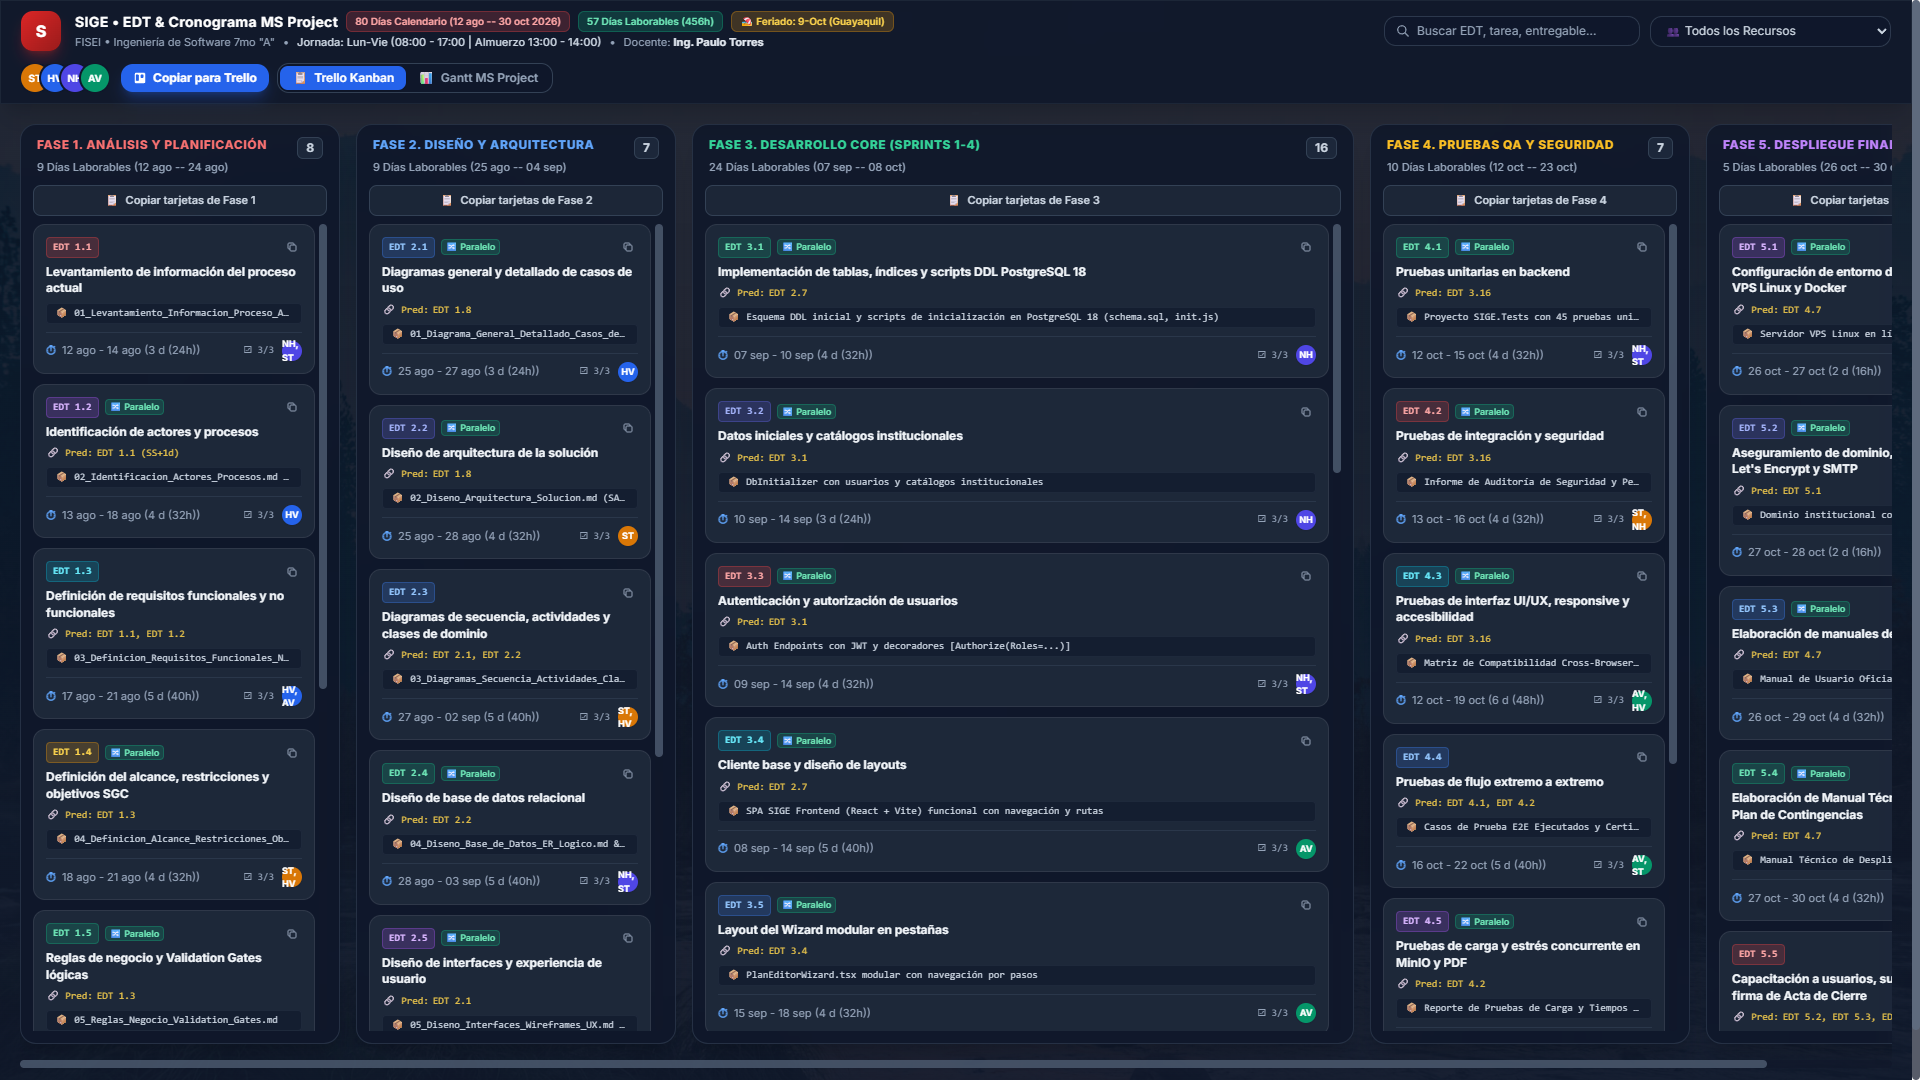
\includegraphics[width=0.88\textwidth,height=5.5cm,keepaspectratio]{images/trello_tablero_captura_real.png}
    \caption{Captura Real del Tablero de Trello: Columna de Fase 1 con 8 Tarjetas 100\% Completadas.}
\end{figure}
\FloatBarrier

\subsection*{Anexo 3: Trazabilidad en Repositorio Institucional Git}
\begin{itemize}[leftmargin=1.5em, itemsep=2pt]
    \item \textbf{Repositorio:} \texttt{FISEI\_Project / SIGE}
    \item \textbf{Rama de Trabajo:} \texttt{main}
    \item \textbf{Commit de Cierre de Fase:} \texttt{f01982a - release(fase1): paquete consolidado de entregables EDT 1.1 a 1.8 y herramientas analiticas}
    \item \textbf{Etiqueta Git (Tag):} \texttt{v0.1-fase1-approved}
    \item \textbf{Archivos Afectados:} 8 documentos técnicos en \texttt{Entregables\_Latex/Fase\_1/}
\end{itemize}


\end{document}
